
\chapter{Introduction}
\label{ch:intro}

\section{Motivation}
Over the past few decades, many algorithms have been developed for different vision problems, \eg, multi-view stereo~\cite{seitz2006comparison,agarwal2011building}, optical flow estimation~\cite{brox2004high,sun2014quantitative}, shape-from-shading~\cite{ikeuchi1981numerical,zhang1999shape}, image matting~\cite{smith1996blue,levin2007closed}, and photometric stereo~\cite{woodham1980ps,hayakawa1994photometric}.
However, these methods often rely on the assumption of a Lambertian surface, and treat the non-Lambertian objects (\eg, transparent and specular objects) as outliers. 

In fact, transparent and specular objects are very common in the real-world (\eg, glass, plastic, and metallic surfaces).
Simply treating them as outliers cannot thoroughly solve the underling problems.
It is important to develop robust methods for analyzing non-Lambertian objects as it enables a more complete and accurate understanding of the captured scene.

Different from a Lambertian surface whose observed brightness is the same from different viewing angles, the appearance of a non-Lambertian surface depends on how it interacts with the environment lights.
The appearance of a transparent object is determined by how it refracts, reflects, absorbs, and scatters the incident light. 
The appearance of a specular object is determined by how it reflects, absorbs, and scatters the incident light.
The complex interaction between the object and environment light increases the difficulties of analyzing transparent and specular objects.

Inspired by the great successes of deep learning based methods in various vision tasks~\cite{lecun1998gradient,krizhevsky2012imagenet,he2016deep}, we propose to take advantage of the powerful feature learning capability of convolutional neural networks (CNNs) and the large scale training data to solve the difficult problems involving non-Lambertian objects.
Specifically, in this thesis, we focus on three vision problems, namely transparent object matting, calibrated photometric stereo, and uncalibrated photometric stereo for non-Lambertian objects.

Traditional image matting methods are tailored for opaque objects. Given an input image, they estimate an object opacity for each pixel (\ie, alpha matte), then the foreground regions can be extracted and composited onto a novel background.
However, object opacity cannot model the refractive effect of a transparent object and thus leads to unrealistic composites (see~\fref{fig:intro_matting} for an example).
Existing methods for transparent object matting often require tedious capturing procedures and long processing time, which limit their practical use.
To address the limitation of the existing alpha matting methods, we introduce a simple and effective deep learning framework to tackle the problem of transparent object matting.

\begin{figure}[tbp] \centering
    \makebox[0.32\textwidth]{(a) Input image} 
    \makebox[0.32\textwidth]{(b) Composite result} 
    \makebox[0.32\textwidth]{(c) Photograph}
    \\
    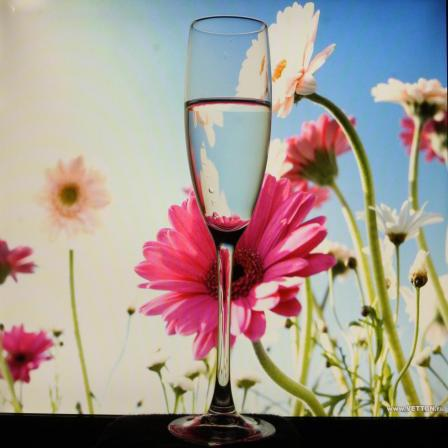
\includegraphics[width=0.32\textwidth]{ch-introduction/images/matting_input}
    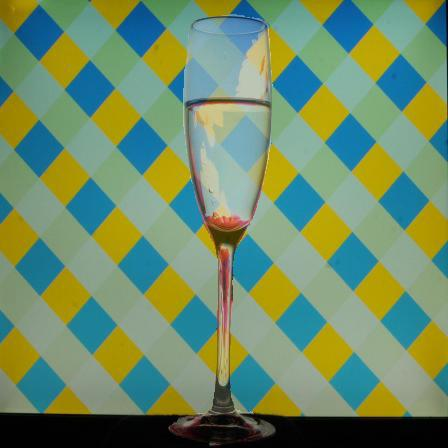
\includegraphics[width=0.32\textwidth]{ch-introduction/images/matting_output}
    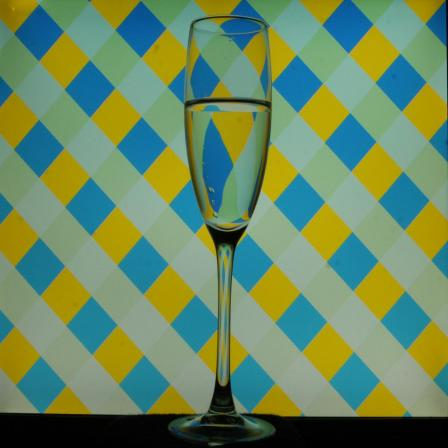
\includegraphics[width=0.32\textwidth]{ch-introduction/images/matting_ref}
    \caption[Example result of the traditional matting method for transparent object]{Example result of the traditional image matting method for transparent object. (a) Input image. (b) Composite result obtained by applying the estimated alpha matte on a novel background. (c) Captured photo of the transparent object in front of the novel background.} \label{fig:intro_matting}
\end{figure}

Photometric stereo aims at recovering the surface normal of a static object from a set of images captured under different light directions~\cite{woodham1980ps,silver1980determining} (see~\fref{fig:intro_ps}).
Compared with multi-view stereo methods, photometric stereo methods use monocular shading cues and naturally avoid the difficult correspondence problem. 
The advantage of photometric stereo is that it can handle specular and textureless surfaces, and can recover highly detailed scene geometry.
However, there are still some limitations in existing photometric stereo methods. (i) Traditional methods often adopt simplified reflectance models to simplify the problem, and this greatly hinders their applications to real-world objects. (ii) Photometric stereo methods typically require calibrated lightings, and the calibration process is often very tedious. There are a few works for uncalibrated photometric stereo, but their performances are far behind the calibrated ones.

In this thesis, we address both these two limitations of existing photometric stereo methods. 
First, we develop a flexible deep learning framework for calibrated photometric stereo. By directly learning a mapping from intensity observations to surface normal, our model can bypass the need for explicitly modeling the surface reflectance model of the object. 
Second, we develop a deep learning method to estimate light directions from the input images, through which we cast the problem of uncalibrated photometric stereo into a calibrated one.

\begin{figure} \centering
    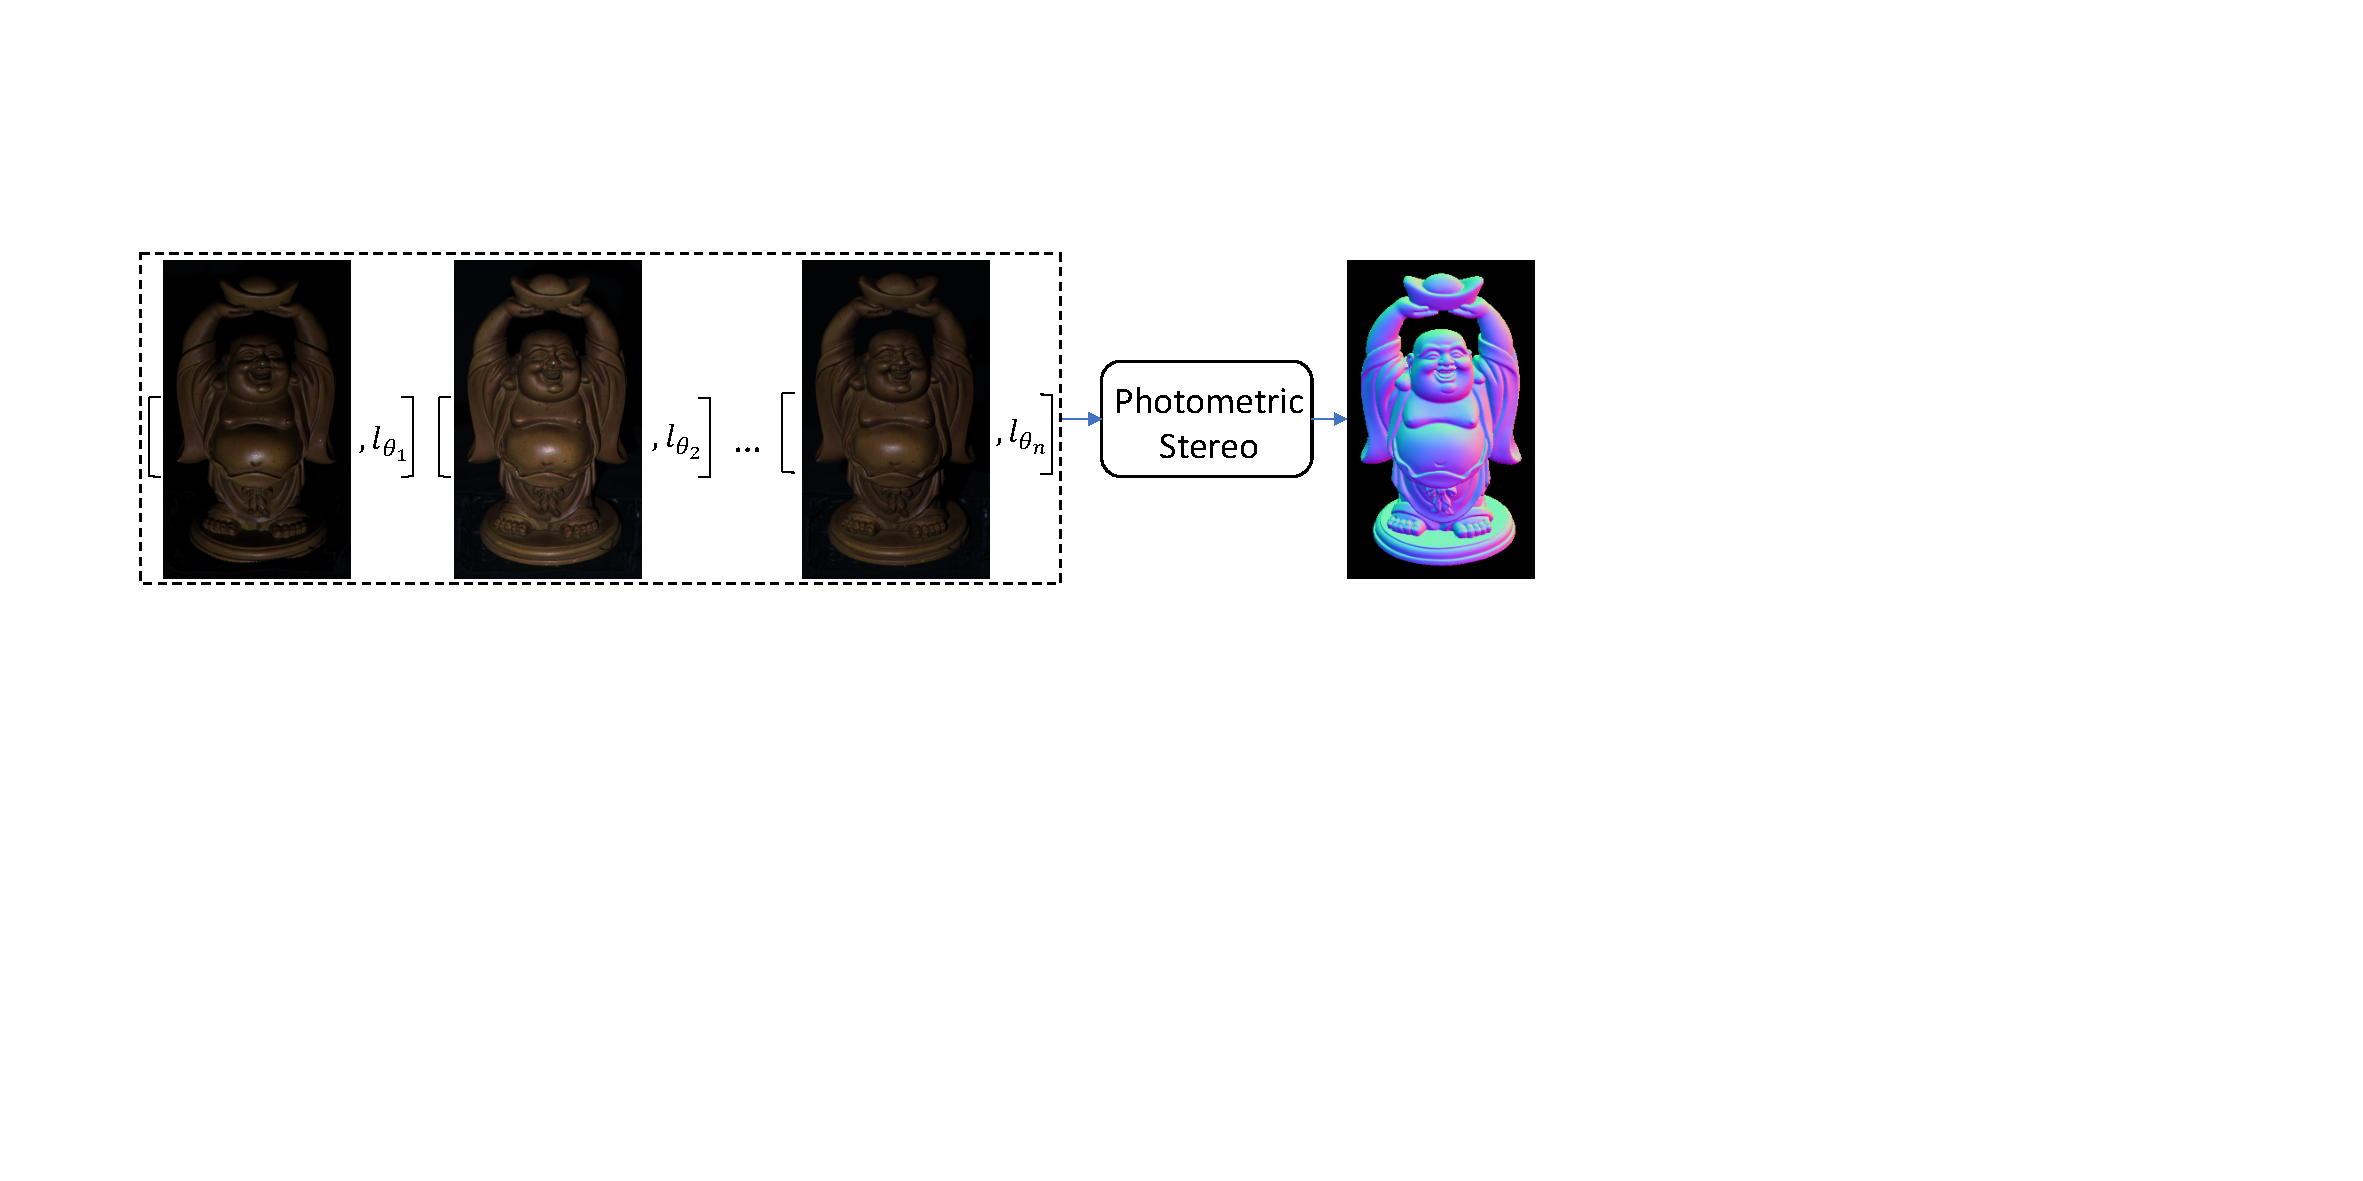
\includegraphics[width=\textwidth]{ch-introduction/images/Intro_PS}
    \caption[Illustration of photometric stereo]{Given multiple images of a static object captured under different light directions, photometric stereo can estimate a surface normal map of the object.} \label{fig:intro_ps}
\end{figure}


\section{Contributions}

The main contributions of this thesis can be summarized as follows:

\begin{itemize}
    \item a convolutional neural network for \textbf{transparent object matting from a single image}. We introduce a simple and efficient model for transparent object matting as simultaneous estimation of an object mask, an attenuation mask, and a refractive flow field. To train and evaluate the proposed method, we create a large-scale synthetic dataset and capture a real dataset as a benchmark for this problem. Preliminary results of this research have been published in~\cite{chen2018tomnet,chen2019learning}

    \item a flexible convolutional neural network for \textbf{calibrated photometric stereo}. Our method directly learns the mapping from reflectance observations to surface normals, and does not depend on a pre-defined set of light directions during training and testing. We introduce two synthetic datasets for learning photometric stereo. Our method outperforms existing methods on multiple real datasets, which demonstrates the effectiveness of the proposed method. Preliminary results of this research have been published in~\cite{chen2018ps,chen2020deepps}.
    \item a convolutional neural network for \textbf{estimating light directions for uncalibrated photometric stereo}. We analyze the features learned by our method, and find that attached shadows, shadings, and specular highlights are key elements for lighting estimation. Based on our findings, we propose an improved method that explicitly utilizes object shape and shading information as guidances for better lighting estimation. Preliminary results of this research have been published in~\cite{chen2019self,chen2020chen_gcnet}.
\end{itemize}

\section{Thesis Outline}
The remainder of this thesis is organized as follows.

\paragraph{\Cref{ch:tomnet}} This chapter addresses the problem of transparent object matting. Existing approaches often require tedious capturing procedures and long processing time, which limit their practical use. In this chapter, we formulate transparent object matting as a refractive flow estimation problem, and propose a deep learning framework, named {\em TOM-Net}, for learning the refractive flow. As no off-the-shelf dataset is available for transparent object matting, we introduce a large-scale synthetic dataset for training, and capture a real dataset for evaluation. 
We then show that our method can be extended to handle cases where a trimap or a background image is available. 
Promising experimental results have been achieved on both synthetic and real data, which clearly demonstrate the effectiveness of our approach.

\paragraph{\Cref{ch:psfcn}} This chapter addresses the problem of calibrated photometric stereo for non-Lambertian surfaces under directional lightings. Existing approaches often adopt simplified reflectance models to make the problem more tractable, but this greatly hinders their applications on real-world objects. 
We propose a deep fully convolutional network, named PS-FCN, that takes an arbitrary number of images of a static object captured under different light directions with a fixed camera as input, and predicts a normal map of the object in a fast feed-forward pass. 
As obtaining ground-truth normal maps of real objects is difficult and time-consuming, we introduce two realistic synthetic datasets for training.
Extensive experiments show that PS-FCN outperforms existing approaches in calibrated photometric stereo.

\paragraph{\Cref{ch:lcnet}} This chapter addresses the problem of lighting estimation for uncalibrated photometric stereo. Previous approaches for this problem often heavily rely on assumptions of specific reflectances and light source distributions.
We first introduce a lighting calibration network, named \emph{LCNet}, that takes an arbitrary number of images as input and estimates their corresponding light directions and intensities.
Surprised by the incredible effectiveness of LCNet, we analyze the features learned by this method and find that they strikingly resemble attached shadows, shadings, and specular highlights. Based on this insight, we propose a guided calibrated network, named \emph{GCNet}, that explicitly leverages object shape and shading information for improved lighting estimation.
Our experiments show that combining our network with existing calibrated photometric stereo methods yields significantly improved results over state-of-the-art uncalibrated methods. 

\paragraph{\Cref{ch:conclusion}} This chapter summarizes the theories and algorithms developed in this dissertation, followed by a brief discussion of potential future work.
